\section{Ejercicio 2: Construyendo Reportes en Power BI - Tarea 2: Crear una Visualización de Mapa a Map Visualization} 

1. At the bottom of the report, click the + icon to add a new page.\\
2. In the Fields pane, in the Customers table, select the City field. Power BI adds a map to the report.\\
3. In the Fields pane, in the Sales table, select the LineTotal field.\\
4. Using the grabber tool on the right side of the chart, resize the map to show all of the bubbles.\\
5. Notice that the bubbles are proportionally sized to represent the data.\\
6. In the Visualizations pane, click Format, and then expand Title.\\
7. In the Title Text box, type World Sales by City, and then click Center.\\

	\begin{center}
	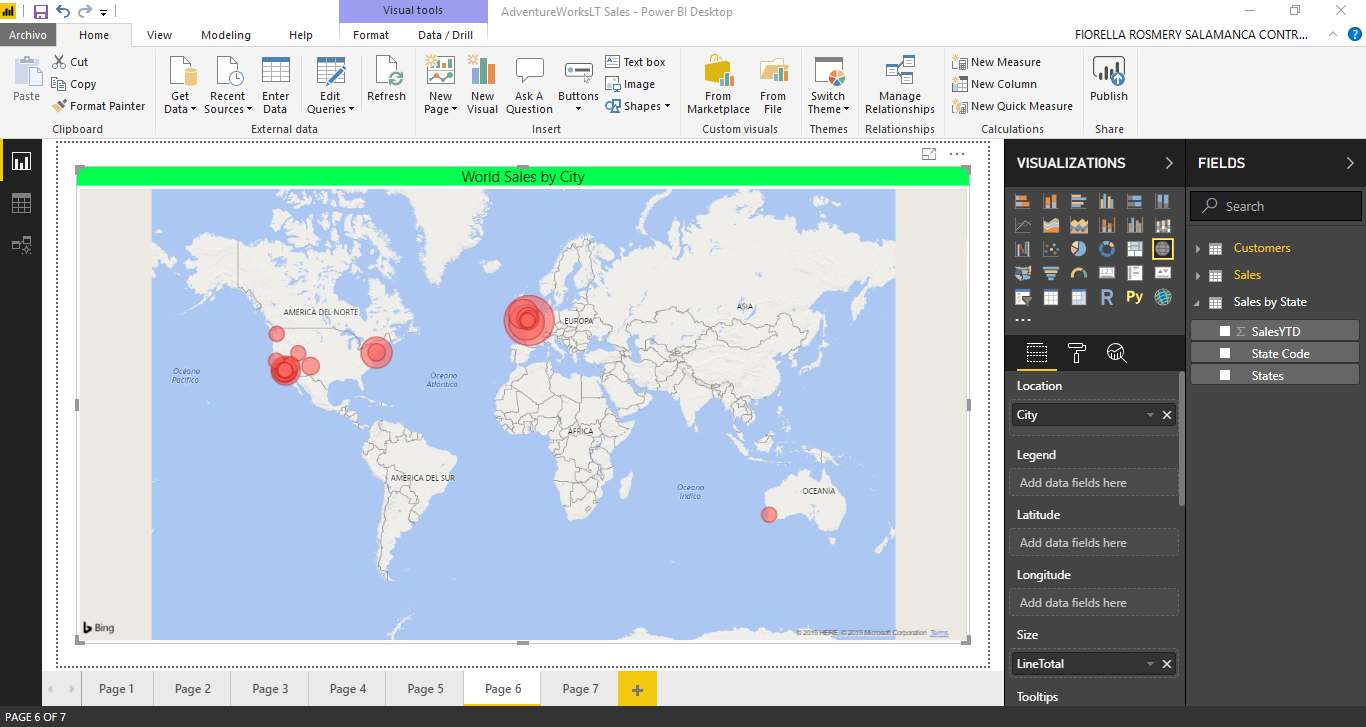
\includegraphics[width=17cm]{./Imagenes/Ejercicio2/Tarea2/1}
	\end{center}	

8. Click the report canvas, and then in the Sales by State table, select the State Code column. Power BI
automatically adds a map.\\
9. In the Sales by State table, select the SalesYTD column.\\
10. In the Visualizations pane, click Filled Map. Using the grabber tool on the right side and at the
bottom of the chart, resize the map to show all the states.\\
11. Notice that the sales cluster in one area.\\
12. Position the cursor on California(CA) to see the sales figure. The value has not been formatted as
currency.\\
13. In the Sales by State table, click the SalesYTD column.\\
14. On the Modeling ribbon, select Format:General, click Currency, and then select \$ English (United
Stated).\\
15. Position the cursor on California(CA) on the map, and notice that the value has been formatted.\\
16. In the Visualizations pane, click Format, and then expand Title.\\
17. In the Title Text box, type Sales by State, and then click Center.\\

	\begin{center}
	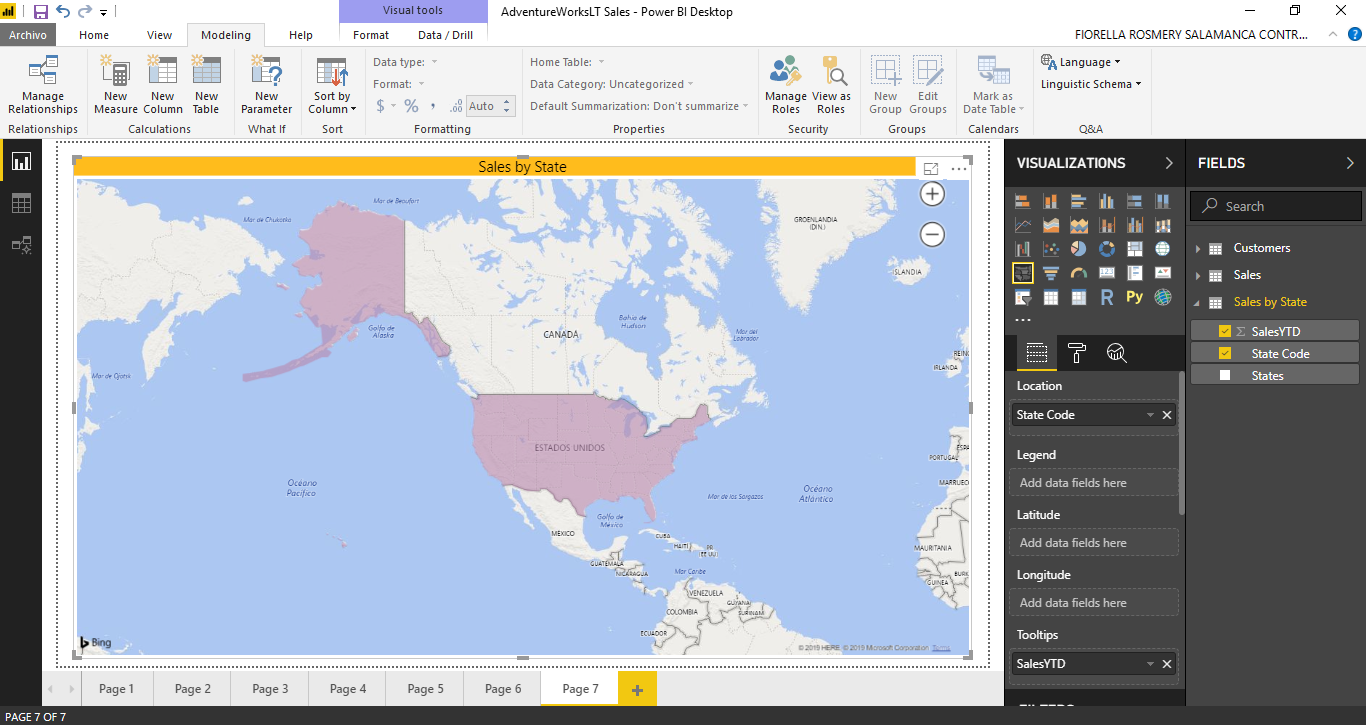
\includegraphics[width=17cm]{./Imagenes/Ejercicio2/Tarea2/2}
	\end{center}	

18. Click Save, and then leave the report open for the next exercise.\\
Results: After this exercise, you should have created a report that has chart visuals and is ready to publish to the Power BI service.